\documentclass[conference]{IEEEtran}
\IEEEoverridecommandlockouts
% The preceding line is only needed to identify funding in the first footnote. If that is unneeded, please comment it out.
\usepackage{cite}
\usepackage{amsmath,amssymb,amsfonts}
\usepackage{algorithmic}
\usepackage{graphicx}
\usepackage{textcomp}
\usepackage{xcolor}
\def\BibTeX{{\rm B\kern-.05em{\sc i\kern-.025em b}\kern-.08em
    T\kern-.1667em\lower.7ex\hbox{E}\kern-.125emX}}
\begin{document}

\title{Microgrid Project\\}

\author{\IEEEauthorblockN{Jesse Both}
\IEEEauthorblockA{\textit{Department of Computer Science and Engineering} \\
\textit{University at Buffalo}\\
Buffalo, New York \\
jessebot@buffalo.edu}}

\maketitle

\begin{abstract}
    ABSTRACT
\end{abstract}

\begin{IEEEkeywords}
Microgrid, Genetic Algorithm
\end{IEEEkeywords}

\section{Introduction}
    Introduction

\section{Design}
    \subsection{Microgrid Block Diagram}
    \begin{figure}[h!]
    \begin{center}
        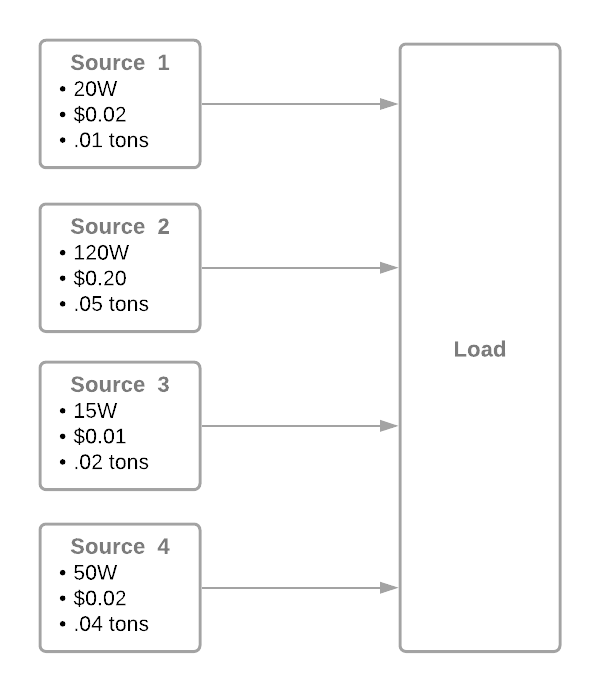
\includegraphics[height=8cm]{graphics/block_diagram.png}
    \end{center}
    \caption{Block Diagram}
    \label{fig:block}
    \end{figure}

    \subsection{Load Time Series}
    This time series was designed by deciding with the idea that the power is being sent to a residential area.  The usage would be low in the middle
    of the night and high when residents are home from work.  It would gradually
    increase/decrease throughout the other parts of the day.  The assumption
    is that a week days are being explored.

    To find the values, a range was given for each hour through out the day.
    A value for each hour within these ranges is randomly selected.  A set
    number of days can be produced.  In order to smooth out the curve an additional parameter was utilized to combine a set of days into a group and take the mean.  The purpose of this is to smooth out the curve into something that would look more realistic.

    \subsection{Source Chromosome Format}
    The chromosome format for each source is
    \[[power, cost, emission]\]

    The gene boundaries are:
    \begin{itemize}
        \item \(15W \leq power \leq 120W\)
        \item \(\$.01 \leq cost \leq \$.2\)
        \item \(.01 tons \leq emission \leq .04 tons\)
    \end{itemize}

    \subsection{Fitness Optimization}
    Economic optimization means that lower cost is better.  If the requirements can be met with lower cost this would be a beneficial economic adjustment.

    Economic boundary for fitness function:
    \textbf{TODO}
    \newline 

    Environmental optimization would imply that less emissions produced would be better for the environment.

    Environmental boundary for fitness function:
    \textbf{TODO}
    \newline 

    Another optimization that is required is the amount of power is delivered.  If there is not enough power being delivered then outages will occur.
    \textbf{TODO}

    \subsection{Defined Constants}
        


\end{document}
